\chapter{評価実験}
\label{chap:experiment}

本章では、本論文で提案する『わかるらんど』のWISS2016での評価実験について述べる。

\newpage

\section{WISS2016での実証実験}
2016年12月14日から16日の3日間開催されたWISS2016において、
プレゼンテーションセッション、デモ中継セッション、招待講演中のコミュニケーションシステムとして
『わかるらんど』を運用する実証実験を行った。
WISS2016では運営が用意したチャットシステム「On-Air Forum」と『わかるらんど』の
2つのコミュニケーションシステムが同時に運用された。
On-Air ForumはWISS2009から毎年運用されており、
『わかるらんど』は今回が初めての運用であった。

\subsection{運用デザイン}
WISS2016では、プレゼンテーションセッション会場の前方に3つのつの大型スクリーンが用意され、
中央のスクリーンを登壇者の発表スライドの表示に、
左のスクリーンをWISS運営が用意したチャットシステムOn-Air Forumの表示に、
右のスクリーンを『わかるらんど』の表示に使用された(図\ref{wiss2016})。
参加者は持参したノートPCから『わかるらんど』にアクセスし利用を行った。
デフォルトで用意したスタンプは図\ref{wiss2016stamp}の33種類である。
会期の半分にあたる2日目の午前までは通常通り『わかるらんど』を運用し、
2日目の午後からは、参加者からの要望により、アカウント名を隠し匿名で投稿する形に変更し運用を行った。

\begin{figure}[h]
\centering
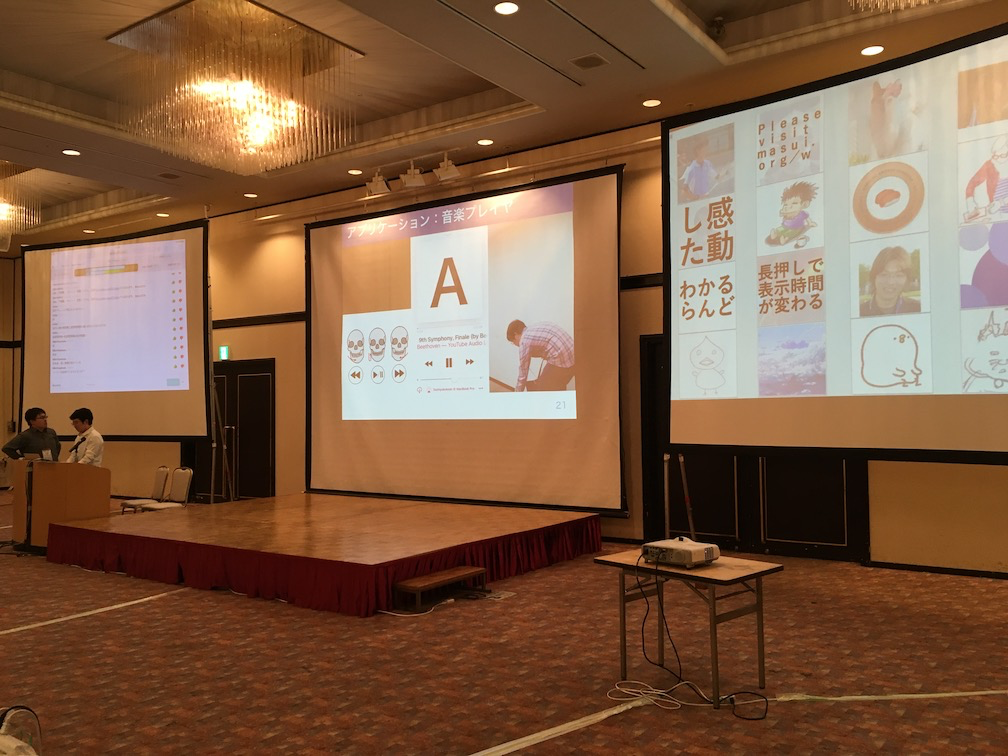
\includegraphics[width=9cm]{images/wiss2016.png}
\caption{WISS2016会場のスクリーン}
\label{wiss2016}
\end{figure}

\begin{figure}[h]
\centering
\fbox{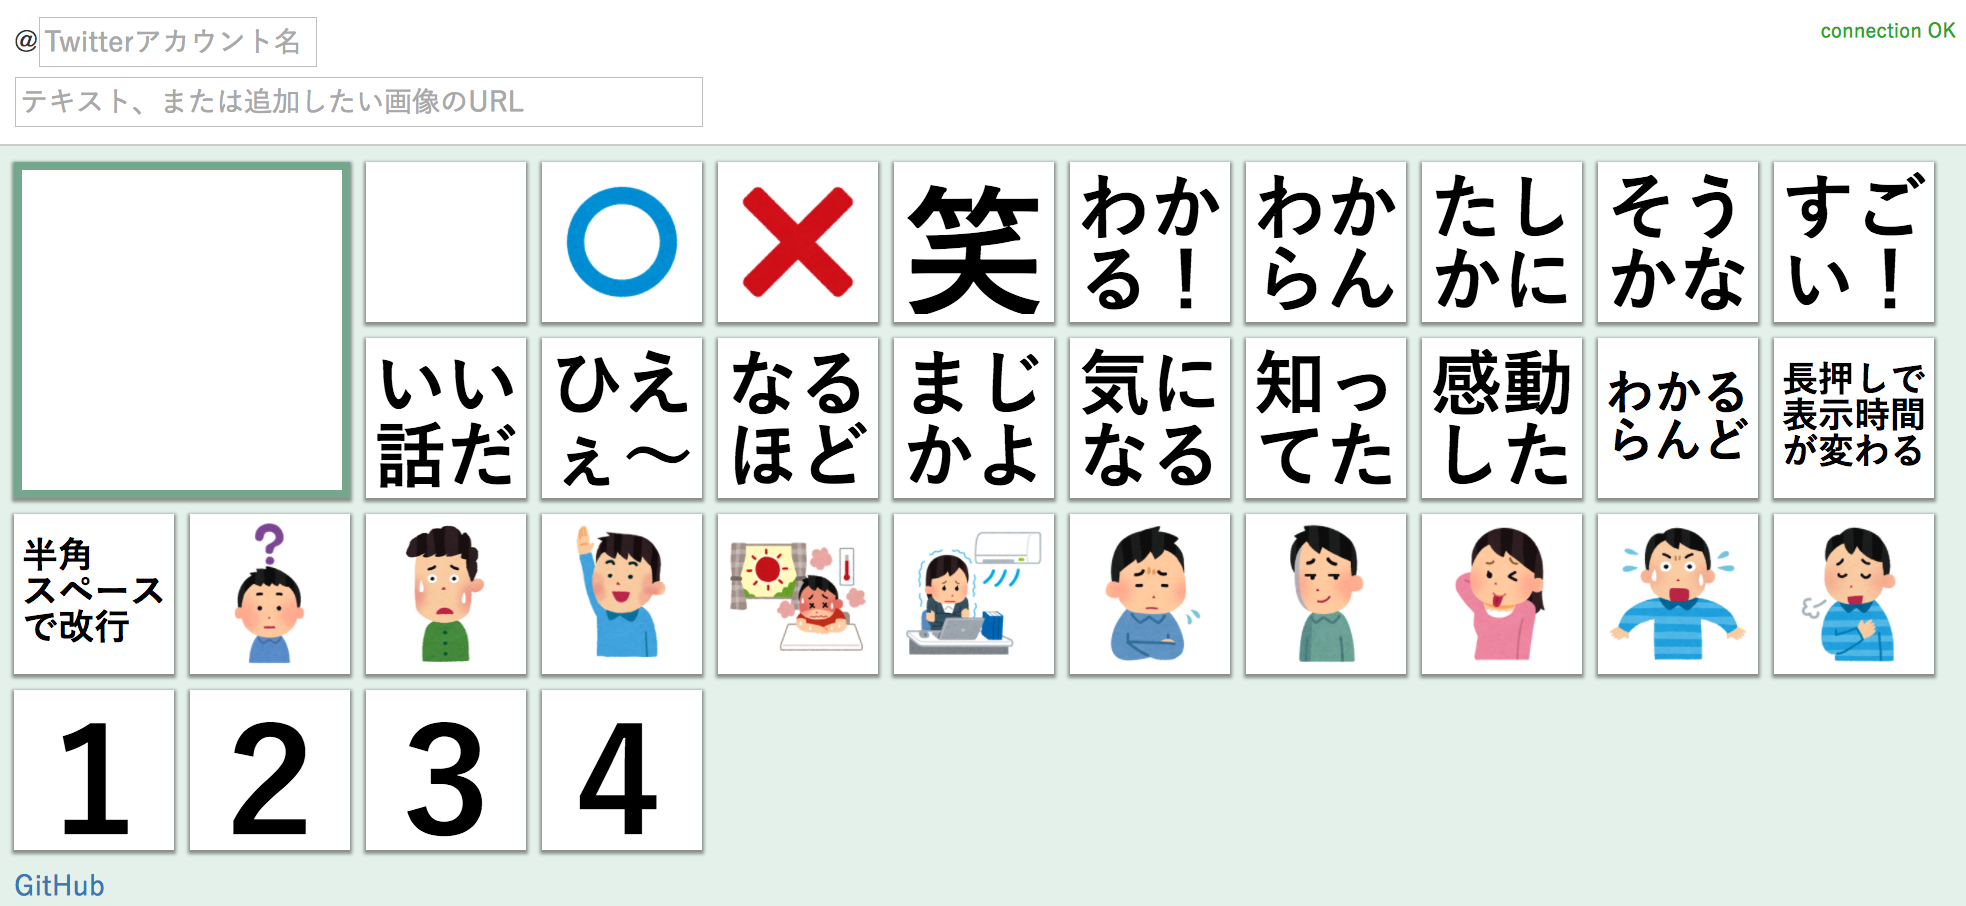
\includegraphics[width=9cm]{images/wiss2016stamp.png}}
\caption{WISS2016の『わかるらんど』でデフォルト用意したスタンプ}
\label{wiss2016stamp}
\end{figure}


\subsection{実験の評価指針}
WISSではこれまでにもさまざまなコミュニケーションシステムが運用されてきた。
しかし、各システムの運用成果報告は一部参加者のコメントを掲載するだけであったり、
システムの各機能が実際にどのように使われたかを観察した結果をまとめたものであったりするなど、
コミュニケーションシステムの定量的な評価手法は確立されていない\cite{nishida2006}\cite{nishida2011}。

今回の運用では、今までWISSで運用されてきたコミュニケーションシステムの運用成果報告と同じく、
『わかるらんど』がどのように利用されたのかを観察した結果をまとめるのに加えて、
定量的な評価としてOn-Air Forumと『わかるらんど』の投稿数を比較した。
学術会議には幅広い年齢層・背景の人が参加するため、
親しい者同士のコミュニケーションよりも精神的な敷居が高くなる。
第3章で述べたように『わかるらんど』のコミュニケーションシステムとしての設計指針は
アウトプットを増やすことであり、
アウトプットと同義である投稿の数を増やすことは本システムの評価に極めて重要である。

\subsection{実験結果}
今回が初めての実験であり過去の実験との比較ができないため、
実験結果は第\ref{chap:wakaruland}で説明した各機能がどのように使われたのかを観察した結果を中心にまとめる。

表\ref{tb:wiss2016experiment}はWISS2016における『わかるらんど』とOn-Air Forumの運用結果である。

\begin{table}[htb]
  \begin{center}
    \caption{WISS2016における『わかるらんど』とOn-Air Forumの運用結果}
    \label{tb:wiss2016experiment}
    \begin{tabular}{|l||r|r|r|} \hline
      システム & 利用人数 & 総投稿数 & 1分あたりの投稿回数 \\ \hline \hline
      わかるらんど & 71人 & 3,781回 & 5.29回 \\ \hline
      On-Air Forum & 99人 & 2,604回 & 3.64回 \\ \hline
    \end{tabular}
  \end{center}
\end{table}

3日間の会期中に全参加者の半分弱にあたる71人が『わかるらんど』で1回以上投稿した。
総投稿数は3,781回で、平均で1分あたり5.29回の投稿があった。

On-Air Forumは全参加者の約6割にあたる99人がログインし、1回以上発言した。
総投稿数は2,604回で、平均で1分あたり3.64回の投稿があった。
ちなみに、前年のWISS2015のOn-Air Forumへの総投稿数は2,948回だった。

これらの結果から、『わかるらんど』の総投稿数はOn-Air Forumの総投稿数よりも多く、
例年On-Air Forumを利用していた人の一部が『わかるらんど』に流れたことを考慮したとしても、
参加者のアウトプットを増やすという要件は満たすことができたといえる。

ユーザごとの発言数を分析すると、『わかるらんど』への投稿の約80\%は
投稿数上位約25\%にあたる18人によって行われており、概ね冪分布になっている。
また、On-Air Forumについても投稿の約80\%は投稿数上位約26\%にあたる26人による投稿で、
同じく冪分布となっていた。
図\ref{wiss2016compare}は『わかるらんど』とOn-Air Forumへの投稿数を対数グラフにプロットしたものである。

\begin{figure}[h]
\centering
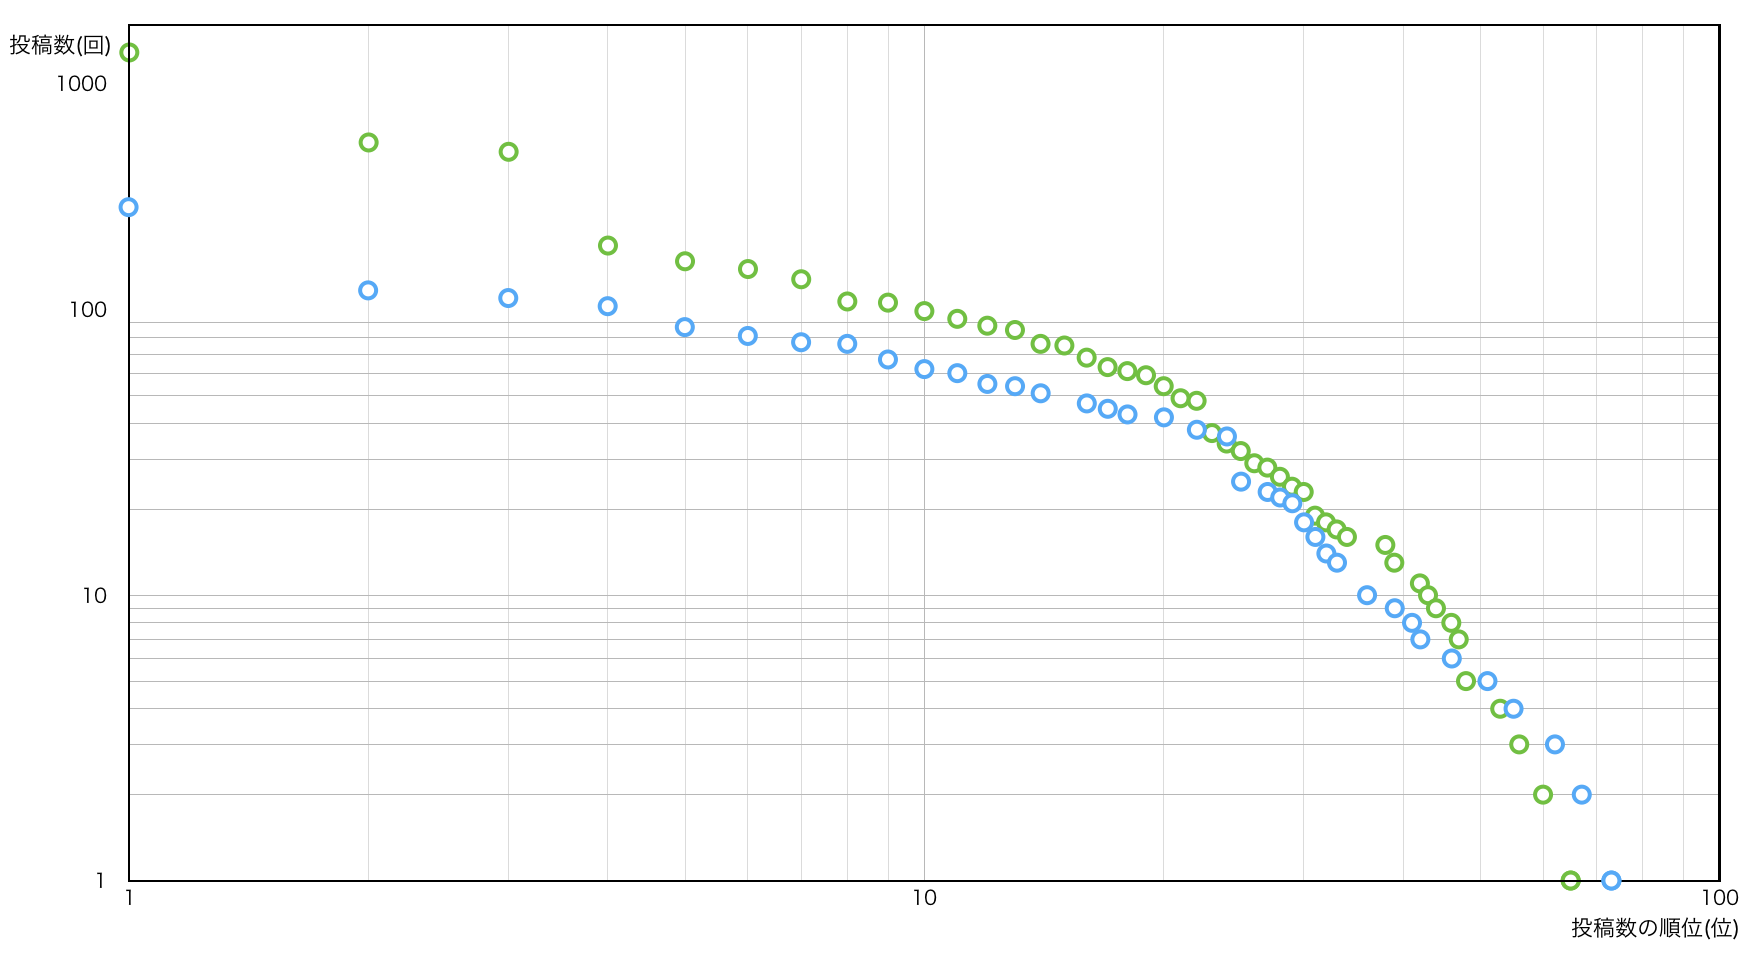
\includegraphics[width=12cm]{images/wiss2016compare.png}
\caption{WISS2016における『わかるらんど』(緑)とOn-Air Forum(青)への投稿のアカウントと発言数の分布}
\label{wiss2016compare}
\end{figure}

さらに詳細な検討によると、会の開始から会期の半分にあたる2日目の午前中までの
『わかるらんど』への投稿数は1,282回であったのに対し、
2日目の午後から3日目の会期終了までの投稿数は2,499回であった。
これは、参加者が『わかるらんど』の使い方に慣れてきたのに加えて、
2日目の午後から適用したアカウント名を隠した匿名化が投稿数の増加に大きく影響したと思われる。

スタンプについては、デフォルトで用意した33種類に加えて525種類のスタンプが作成され、
会期中に投稿されたスタンプは558種類であった。
最も多く使われたスタンプは「笑」で141回投稿された。
2番目に多く使われたスタンプは「👏」、3番目は「なる ほど」であった。
「笑」は発表者が取りに行った時や、
予想だにしないアクシデントがあった時などに使用されていた。
「👏」は発表が終わった時に発表者に対して拍手をするタイミングで投稿されていた。
「なる ほど」は汎用性の高い相槌として、発表中に満遍なく使用されていた。

また、発表中に「ポケモンGo\footnote{http://www.pokemongo.jp}」の話題が出た時や
「自由形状の竹とんぼのインタラクティブデザインシステム」の発表では、
ポケモンに関するスタンプ\ref{pokemon}や竹トンボを飛ばす少年のスタンプ\ref{taketombo}
などを誰かが『わかるらんど』に投稿し、他の参加者がそのスタンプをコピーして使用する
という使われ方が見られた。

\begin{figure}[h]
\centering
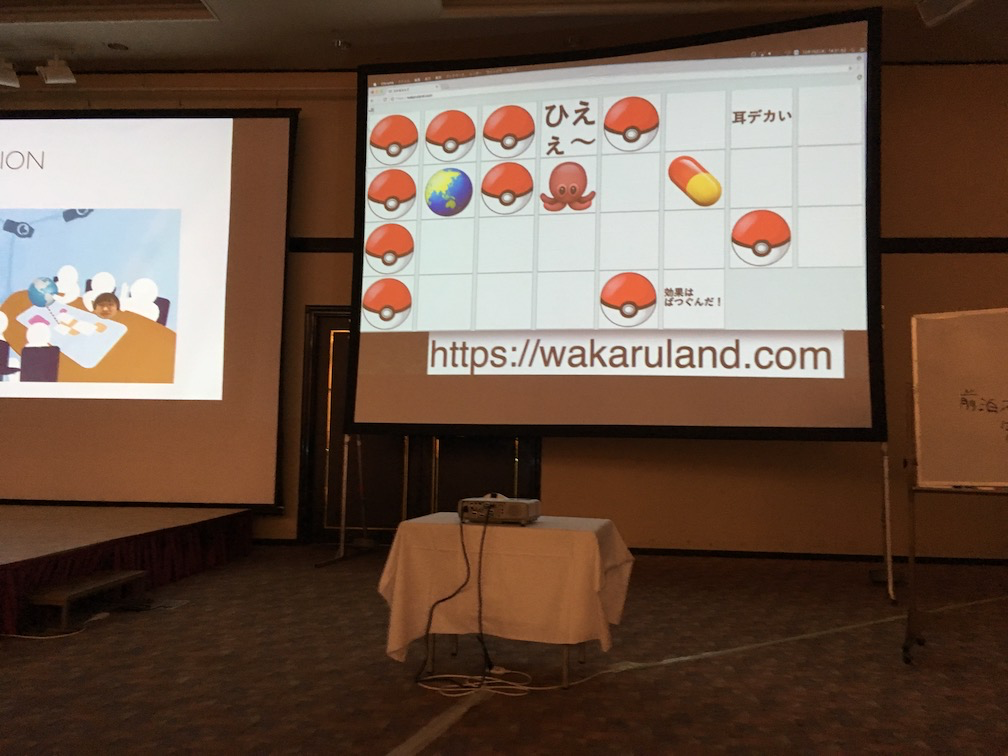
\includegraphics[width=11cm]{images/pokemon.png}
\caption{沢山投稿されるモンスターボールのスタンプ}
\label{pokemon}
\end{figure}

\begin{figure}[h]
\centering
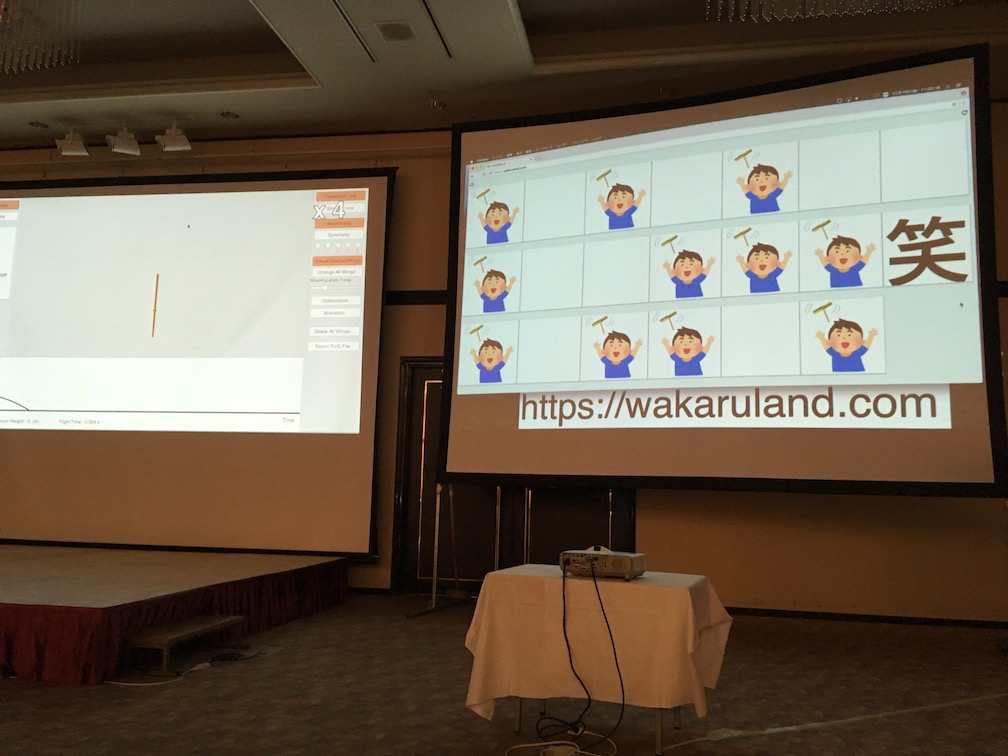
\includegraphics[width=11cm]{images/taketombo.png}
\caption{沢山投稿される竹トンボを飛ばす少年のスタンプ}
\label{taketombo}
\end{figure}


\section{研究室においての利用}
筆者の研究室では,
約6ヶ月の間『わかるらんど』を研究室内の大型ディスプレイに表示して実際に利用してきた.
筆者の研究室ではWebLindaを使用して,
Web情報やArduinoやRaspberry Piに接続したセンサ情報を利用し,
\begin{itemize}
\item 部屋の明るさを知る
\item 部屋の温度を知る
\item 風速と風向を知る
\item 入口のドアの鍵を開ける
\item 部屋の照明を点ける/消す
\end{itemize}
といったことをSlack\footnote{https://slack.com}のチャットボットを通じて行える
IoT環境を構築している(図\ref{slack})が,『わかるらんど』と組み合わせることで
さらに便利に使うことができた.

\begin{figure}[h]
\centering
\fbox{
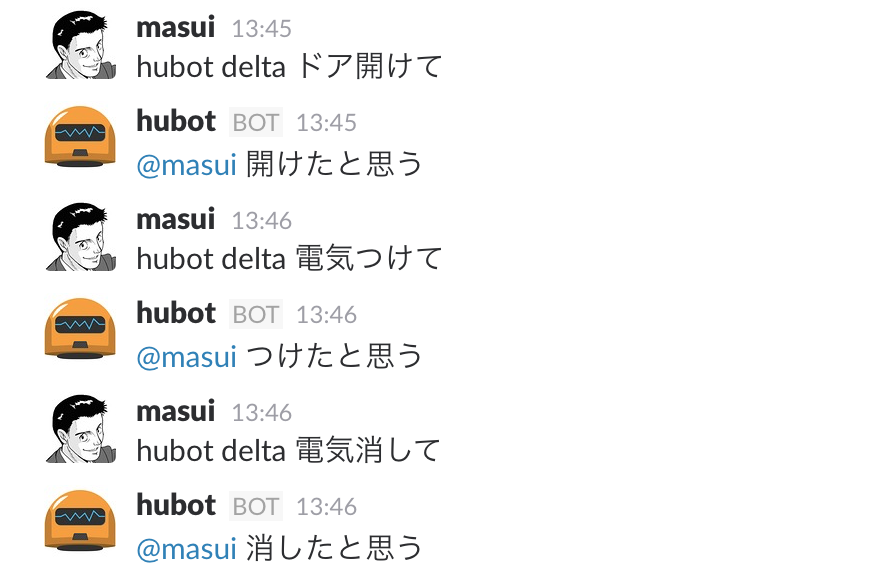
\includegraphics[width=9cm]{images/slack.png}
}
\caption{SlackのチャットボットによるIoT機器の操作}
\label{slack}
\end{figure}

図\ref{light}は部屋の明るさを表示するデータセルだが,
明るさのデータの値が小さい時は\texttt{background}画像を変更することで,
照明が点いているのか消えているのかがわかるようになった.

\begin{figure}[h]
\centering
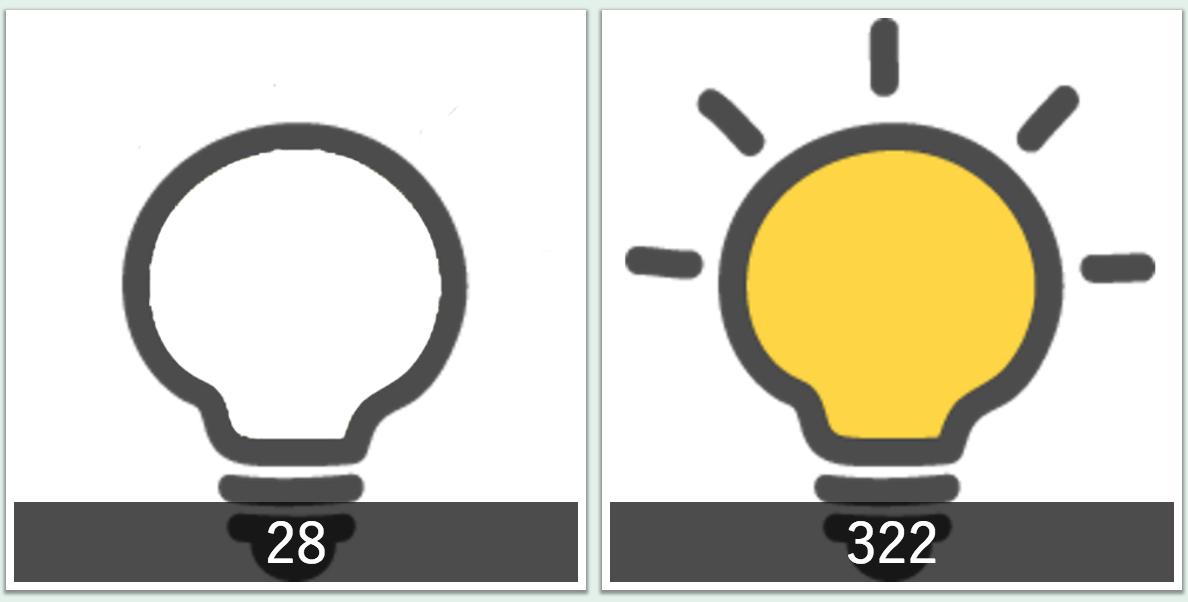
\includegraphics[width=9cm]{images/light.png}
\caption{照明が消えている時(左)と点いている時(右)}
\label{light}
\end{figure}

図\ref{door}は,研究室のドアが最後に開いた時間を表示するデータセルである.
普段は扉の画像を\texttt{background}にしているが,
実際に扉が開いた時に10秒間だけ\texttt{background}を図\ref{door}右のように
扉を開ける人の画像にすることで,誰かが入室したことが視覚的にわかるようになった.

\begin{figure}[h]
\centering
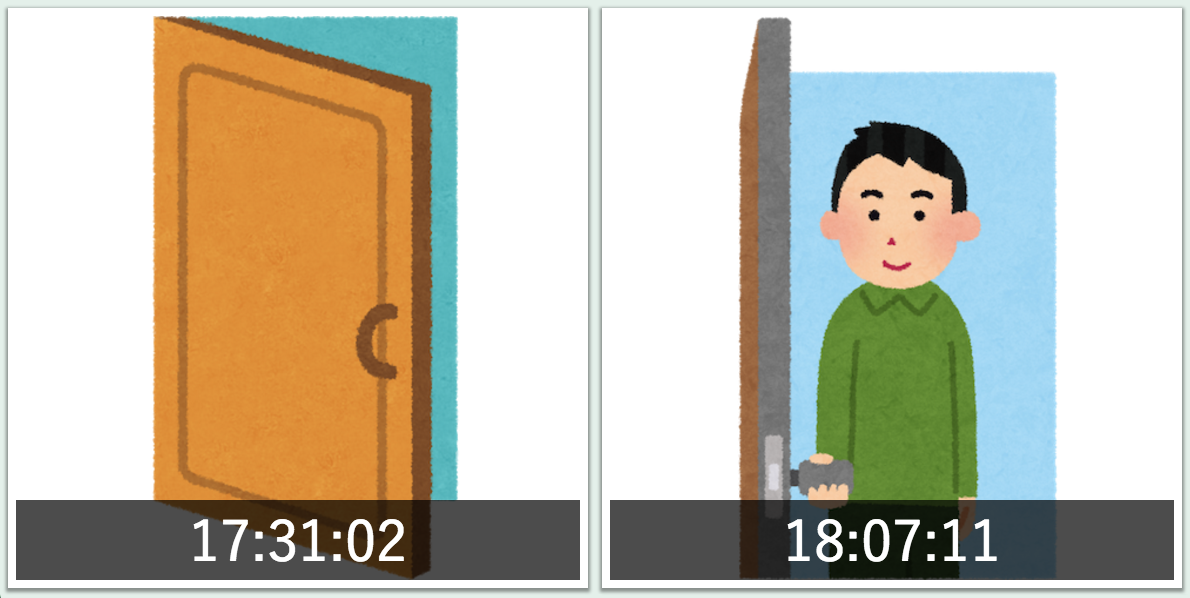
\includegraphics[width=9cm]{images/door.png}
\caption{ドアの普段の表示(左)と誰かが入室した時(右)}
\label{door}
\end{figure}

ミーティングの時間には積極的に『わかるらんど』を利用し,
普段発言の少ない人でも何らかの反応を表明したり,
発表者が聴衆の反応をひと目で把握することができるようになった.
発表中に『わかるらんど』に「わからん」というリアクションが並んだときは,
発表者が詳しい説明をすることができたり,
誰かが面白いことを言ったときに「笑」というリアクションが並び,
『わかるらんど』を通じて一体感が生まれたりすることもあった(図\ref{wara}).

\begin{figure}[h]
\centering
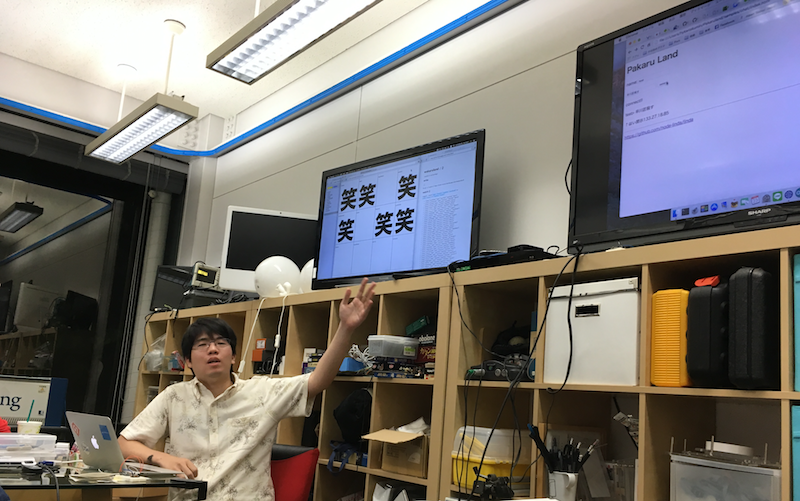
\includegraphics[width=9cm]{images/wara.png}
\caption{『わかるらんど』を使用したミーティング}
\label{wara}
\end{figure}

また,コンピュータで何か別の作業をしているときに,
Webブラウザで『わかるらんど』を開いてリアクションするのが面倒であるという意見もあった.
そこで,図\ref{heebutton}や図\ref{10key}のような
独自の『わかるらんど』入力ハードウェアを作成した.
これらを利用することで,限られたリアクションではあるが,
Webブラウザを開くことなく『わかるらんど』にリアクションを表示することができるようになった.

\begin{figure}[h]
\centering
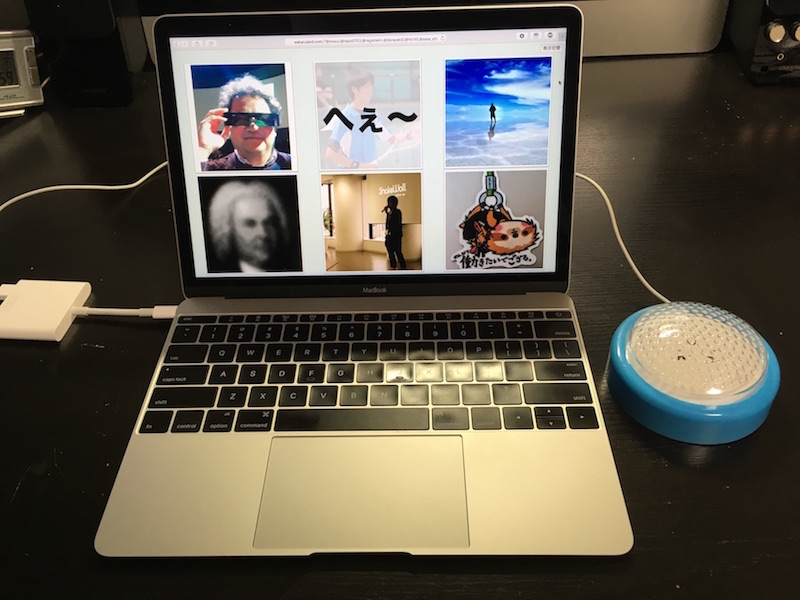
\includegraphics[width=8cm]{images/heebutton.png}
\caption{押すと「へぇ〜」とリアクションできるボタン}
\label{heebutton}
\end{figure}

\begin{figure}[h]
\centering
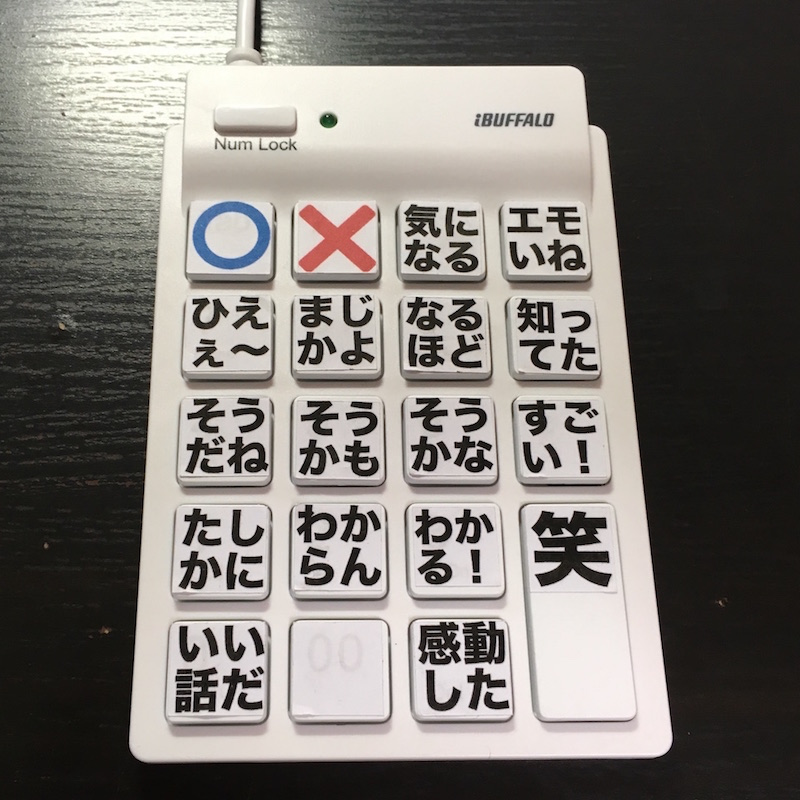
\includegraphics[width=7cm]{images/10key.png}
\caption{テンキーを利用した入力装置}
\label{10key}
\end{figure}